\documentclass[usenames,dvipsnames]{article}

%\renewcommand{\familydefault}{\sfdefault}

\usepackage{standalone}
\usepackage{pdfpages}
\usepackage{upgreek}
\usepackage[english]{babel}
\usepackage{geometry}

\usepackage{color}
\usepackage{xcolor}
\usepackage{float}
\usepackage{tabularx}
\usepackage{booktabs}
\usepackage{pgfplots}
\usepackage{amsmath}
\usepackage{listings}
\usepackage{amssymb}
\usepackage{amsfonts}
\usepackage{siunitx}
\usepackage{tikz}
\usepackage{graphics} % for pdf, bitmapped graphics files
\usepackage{graphicx}
\usepackage{exsheets}
\usepackage{exsheets-listings}
\usepackage{cprotect}
\usepackage{algorithm}
\usepackage{algorithmicx}
\usepackage[noend]{algpseudocode}
\usepackage[pdfusetitle]{hyperref}
\usepackage[shortlabels]{enumitem}
\usepackage{filecontents}
\usepackage{multirow}
\usepackage{multicol}
\usepackage{setspace}
\usepackage{xparse}
\usepackage{fancyhdr}
\usepackage{datetime}
\usepackage{totcount}
\usepackage{fancyvrb}
\usepackage{minted}
% Needed to manage fonts
\ifxetex
  \usepackage{fontspec}
  % To support LaTeX quoting style
  \defaultfontfeatures{Ligatures=TeX}
\else
  \usepackage[LGR, T1]{fontenc}
  % Replace by the encoding you are using
  \usepackage[utf8x]{inputenx}
\fi
% Needed to manage math fonts
%\usepackage{unicode-math}
%\renewcommand{\familydefault}{\sfdefault}
% Needed to use icons from font-awesome
% (https://github.com/posquit0/latex-fontawesome)
\usepackage{fontawesome}

%\usepackage{../partials/fontawesome5}

%\usepackage{fontawesome}
%\usepackage{fontawesome5}
%\usepackage{academicons}


\usetikzlibrary{backgrounds,patterns,arrows,arrows.meta,calc,intersections,shapes,positioning,decorations.pathreplacing,decorations.markings,decorations.pathmorphing}
\usepackage{multicol}
\usepackage{subcaption}
\input{partials/setup}
\input{partials/styles}

\renewcommand{\familydefault}{\rmdefault}

%YOUR NAME HERE
\newcommand{\studentname}{Asem Mohamed Alaaeldin}
%YOUR SECTION HERE INSTEAD OF 0
\newcommand{\SN}{ 0 }
%YOUR BENCH NUMBER HERE INSTEAD OF 0
\newcommand{\BN}{ 0 }


\author{\studentname ~ Sec. \SN ~ BN. \BN}
\date{Sunday 12\textsuperscript{th} April, 2020}
\title{Data Structures and Algorithms [SBE201] (Spring 2020)\\ Report 1\\~\\
{\small  Linked Lists }}

\makeatletter
\@addtoreset{question}{section}
  
\hypersetup{
    pdfauthor={{Asem Alaa}},
    pdftitle={{\@title}},
    pdfsubject={Data Structures and Algorithms [SBE201] (Spring 2020)},
    pdfkeywords={Report 1, Linked Lists}
    }
    
\makeatother


\begin{document}

\maketitle

\newminted{cpp}{bgcolor=Black,frame=lines,framesep=2mm,baselinestretch=1.2,linenos}

\section{Problem Set}

\subsection{Linked List Size}




\cprotEnv \begin{question}
\begin{cppcode}
struct IntegerNode
{
  int data;
  IntegerNode *next;
};

int size( IntegerNode *front )
{

}
\end{cppcode}

\begin{enumerate}[A)]
\item Implement the function \CppVerb{size} that returns the size of a given linked list (count of elements).
\item Provide a time complexity estimate using the Big-O notation.
\item Can you provide a recursive version of the \CppVerb{size} function?
\end{enumerate}
\end{question}

\cprotEnv \begin{solution}

\begin{enumerate}[A)]
\item  \mbox{}\\

\begin{cppcode}
int size( IntegerNode *front )
{
  int count = 0;
  auto tempt = front;
  while( temp != nullptr ) 
  {
    ++count;
    temp = temp->next;
   }
  else count;
}
\end{cppcode}
\item $O(n)$
\item \mbox{}\\
\begin{cppcode}
int size( IntegerNode *front )
{
  if( front == nullptr ) return 0;
  else return 1 + size( front->next );
}
\end{cppcode}
\end{enumerate}


\end{solution}


\subsection{Linked List Operations}




\cprotEnv \begin{question}
\begin{cppcode}
#include <iostream>
struct IntegerNode
{
  int data;
  IntegerNode *next;
};
void funx(node* front)
{
  if(front == nullptr) return;
  fun1(front->next);
  std::cout << front->data << " ";
}
\end{cppcode}

\begin{enumerate}[A)]
\item What does the function \CppVerb{funx} do?
\item What is the output would be if the input linked list is represented in order as: \CppVerb{5->90->300->7->55}
\item What is the time complexity of such a function.
\end{enumerate}
\end{question}

\begin{solution}

\begin{enumerate}[A)]
\item prints the elements of the LL in \textbf{reversed order}.
\item \CppVerb{"55 7 300 90 5"}
\item $O(n)$
\end{enumerate}

\end{solution}



\subsection{Doubly-Linked List}



\cprotEnv \begin{question}
\begin{cppcode}
struct IntegerNode
{
  int data;
  IntegerNode *next;
  IntegerNode *back;
};

struct IntegersLL
{
  IntegerNode *front;
};

void insertAt( IntegersLL &list , int index, int data )
{
  
}
\end{cppcode}
\begin{enumerate}[A)]
\item Implement a function \CppVerb{insertAt} to insert an element at arbitrary \CppVerb{index} in a \textbf{linked list}.
\item Provide a visual illustratoin to the steps in order to support that operation.
\end{enumerate}
\end{question}
\cprotEnv \begin{solution}

\begin{enumerate}[A)]
\item  \mbox{}\\
\begin{cppcode}
void insertAt( IntegersLL &list , int index, int data )
{
  auto temp = list.front;
  for( int i = 0; i < index; ++i ) temp = temp->next;
  auto node = new IntegerNode{ data , temp , temp->prev };
  if( temp->next ) temp->next->prev = node;
  if( temp->prev ) temp->prev->next = node;
}
\end{cppcode}

\item 

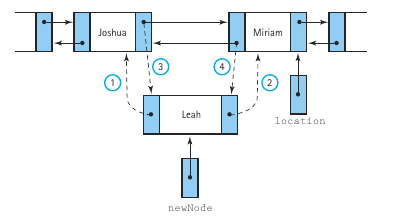
\includegraphics{imgs/insertAt.png}


\end{enumerate}

\end{solution}


\subsection{Circular Linked List}





\cprotEnv \begin{question}
\begin{cppcode}
struct IntegerNode
{
  int data;
  IntegerNode *next;
};

struct IntegersLL
{
  IntegerNode *front;
};

void pushFront( IntegerLL &list, int data )
{
    list.front = new node{ data , list.front };
}

node *backNode( IntegerLL &list )
{
    node *temp = list.front;
    while( temp->next != nullptr )
        temp = temp->next;
    return temp;
}

void *pushBack( IntegerLL &list, double data )
{
    if( list.front == nullptr )
        return pushFront( list , data );
    else
    {
        node *back = backNode( list );
        back->next = new node{ data , nullptr };
    }
}

void removeBack( IntegerLL &list )
{ 
    if( isEmpty( list ))
        return;
    else if( list.front->next == nullptr )
        removeFront( list );
    else
    {
        IntegerNode *prev = list.front;
        while( prev->next->next != nullptr )
            prev = prev->next;
        delete prev->next;
        prev->next = nullptr;
    }
}

void printLL( IntegerLL &list )
{
    node *current = list.front;
    while( current != nullptr )
    {
        std::cout << current->data;
        current = current->next;
    }
}
\end{cppcode}

The functions: \CppVerb{pushFront}, \CppVerb{backNode}, \CppVerb{pushBack}, \CppVerb{removeBack}, and \CppVerb{printLL} are a implemented earlier for a regular linked list.
How would you change each function to work properly for a circular linked list that uses only a \textbf{front} pointer.
\end{question}

\begin{solution}

\begin{itemize}
\item Check \href{https://github.com/sbme-tutorials/sbme-tutorials.github.io/blob/master/2020/data-structures/snippets/report1/cdll/main.cpp}{an implementation of circular doubly-linked list (template class)}
\item Check \href{https://github.com/sbme-tutorials/sbme-tutorials.github.io/blob/master/2020/data-structures/snippets/report1/cll/main.cpp}{an implementation of circular singly-linked list (template class)}

\end{itemize}
\end{solution}

\end{document}
